% Q12
\question The actual area of a playground is $900\text{ m}^2$ . If the area of the playground on a map is $36\text{ cm}^2$ , then the scale of the map is
\begin{choices}
    \choice $1 : 25$ .
    \choice $1 : 50$ .
    \correctchoice $1 : 500$ .
    \choice $1 : 250\,000$ .
\end{choices}
\begin{solution}
\[ \frac{36\text{ cm}^2}{900\text{ m}^2} = \frac{36\text{ cm}^2}{900 \times (100\text{ cm})^2} = \frac{1}{250\,000} = \left(\frac{1}{500}\right)^2 \]
Thus, the scale of the map is $1 : 500$ (C).
\end{solution}

% Q13
\question It is given that $z$ varies directly as $x$ and inversely as $\sqrt{y}$ . If $y$ is decreased by $64\%$ and $z$ is increased by $25\%$ , then $x$
\begin{choices}
    \choice is increased by $20\%$ .
    \choice is increased by $80\%$ .
    \correctchoice is decreased by $25\%$ .
    \choice is decreased by $75\%$ .
\end{choices}
\begin{solution}
Since $z = \dfrac{kx}{\sqrt{y}}$, we have $x = \dfrac{z\sqrt{y}}{k}$. \\
New value of $x$:
\[ x_{\text{new}} = \frac{(1.25z)\sqrt{0.36y}}{k} = 1.25(0.6)x = 0.75x = (1 - 25\%)x \]
Thus, $x$ is decreased by $25\%$ (C).
\end{solution}

% Q16
\question In the figure, the diameter of the semicircle $ABC$ is $3\text{ cm}$ . If $AC = 2\text{ cm}$ , find the area of the shaded region correct to the nearest $0.01\text{ cm}^2$ .

\begin{minipage}{0.45\textwidth}
\begin{choices}
    \choice $0.23\text{ cm}^2$
    \correctchoice $0.52\text{ cm}^2$
    \choice $0.64\text{ cm}^2$
    \choice $1.07\text{ cm}^2$
\end{choices}
\end{minipage}
\begin{minipage}{0.52\textwidth}
\centering
\begin{tikzpicture}[scale=0.9]
    \def\R{2.25}
    \coordinate (O) at (0,0);
    \coordinate (A) at (180:\R);
    \coordinate (B) at (0:\R);
    \coordinate (C) at (96.38:\R);
    \fill[pattern=north east lines] (A) arc (180:96.38:\R) -- cycle;
    \draw[thick] (B) arc (0:180:\R) -- cycle;
    \draw[thick] (A) -- (C);
    \node[below left] at (A) {$A$};
    \node[below right] at (B) {$B$};
    \node[above] at (C) {$C$};
\end{tikzpicture}
\end{minipage}
\begin{solution}
Let $O$ be the centre of the semicircle ($OA = OC = 1.5\text{ cm}$). By the cosine formula in $\triangle OAC$:
\[ \cos\angle AOC = \frac{1.5^2 + 1.5^2 - 2^2}{2(1.5)(1.5)} = \frac{1}{9} \implies \angle AOC \approx 83.62^\circ \]
Area of the shaded segment $= \pi(1.5)^2 \times \dfrac{83.62^\circ}{360^\circ} - \frac{1}{2}(1.5)^2\sin 83.62^\circ \approx 0.52\text{ cm}^2$ (B).
\end{solution}

% Q17
\question In the figure, the solid consists of a right circular cone and a hemisphere with a common base. The base radius and the height of the circular cone are $3\text{ cm}$ and $4\text{ cm}$ respectively. Find the total surface area of the solid.

\begin{minipage}{0.45\textwidth}
\begin{choices}
    \choice $30\pi\text{ cm}^2$
    \correctchoice $33\pi\text{ cm}^2$
    \choice $48\pi\text{ cm}^2$
    \choice $51\pi\text{ cm}^2$
\end{choices}
\end{minipage}
\begin{minipage}{0.52\textwidth}
\centering
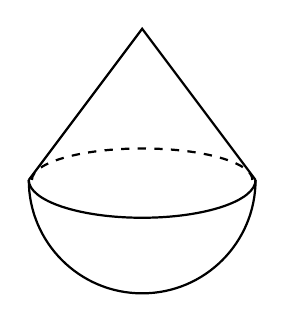
\begin{tikzpicture}[scale=0.8]
    \draw[thick] (-1.8,0) arc (180:360:1.8 and 0.6);
    \draw[thick,dashed] (1.75,0) arc (0:180:1.75 and 0.5);
    \draw[thick] (-1.8,0) arc (180:360:1.8);
    \draw[thick] (-1.8,0) -- (0,2.4) -- (1.8,0);
\end{tikzpicture}
\end{minipage}
\begin{solution}
The slant height of the cone is $\sqrt{3^2 + 4^2} = 5\text{ cm}$. \\
Total surface area $= \pi(3)(5) + 2\pi(3)^2 = 15\pi + 18\pi = 33\pi\text{ cm}^2$ (B).
\end{solution}

% Q18
\question In the figure, $ABCD$ is a trapezium with $AD \parallel BC$ and $AD : BC = 2 : 3$ . Let $E$ be the mid-point of $BC$ . $AC$ and $DE$ intersect at $F$ . If the area of $\triangle CEF$ is $36\text{ cm}^2$ , then the area of the trapezium $ABCD$ is

\begin{minipage}{0.45\textwidth}
\begin{choices}
    \choice $216\text{ cm}^2$ .
    \choice $264\text{ cm}^2$ .
    \correctchoice $280\text{ cm}^2$ .
    \choice $320\text{ cm}^2$ .
\end{choices}
\end{minipage}
\begin{minipage}{0.52\textwidth}
\centering
\begin{tikzpicture}[scale=0.8]
    \coordinate (B) at (0,0);
    \coordinate (E) at (2.4,0);
    \coordinate (C) at (4.8,0);
    \coordinate (A) at (1.2,3.0);
    \coordinate (D) at (4.4,3.0);
    \path[name path=AC] (A) -- (C);
    \path[name path=DE] (D) -- (E);
    \path[name intersections={of=AC and DE, by=F}];
    \draw[thick] (A) -- (B) -- (C) -- (D) -- cycle;
    \draw[thick] (A) -- (C);
    \draw[thick] (D) -- (E);
    \node[above left] at (A) {$A$};
    \node[below left] at (B) {$B$};
    \node[below] at (E) {$E$};
    \node[below right] at (C) {$C$};
    \node[above right] at (D) {$D$};
    \node[above] at (F) {$F$};
\end{tikzpicture}
\end{minipage}
\begin{solution}
Since $AD : BC = 2 : 3$ and $EC = \frac{1}{2}BC$, we have $AD : EC = 4 : 3$. \\
Since $\triangle ADF \sim \triangle CEF$, we have $\text{Area}(\triangle ADF) = 36 \times \left(\frac{4}{3}\right)^2 = 64\text{ cm}^2$ and $\text{Area}(\triangle CDF) = 36 \times \frac{4}{3} = 48\text{ cm}^2$. \\
Thus $\text{Area}(\triangle ACD) = 64 + 48 = 112\text{ cm}^2$ and $\text{Area}(\triangle ABC) = \frac{3}{2}(112) = 168\text{ cm}^2$. \\
Area of trapezium $ABCD = 112 + 168 = 280\text{ cm}^2$ (C).
\end{solution}